\section{APX-completeness for segments parallel to axes}
\label{section:segment_apx}

In this section we analyze whether there exists 
PTAS for geometric set cover for rectangles.
We show that we can restrict this problem
to a very simple setting:
segments parallel to axes and allow (1/2)-extension,
and the problem is still APX-hard.
Note that segments are just degenerated rectangles
with one side being very narrow.


Our results can be summarized in the following
theorem and this section aims to prove it.

\begin{tw}{
\label{segment_cover_apx_hard}
	\textbf{(axis-parallel segment set cover with 1/2-extension is APX-hard)}.	
	Unweighted geometric set cover
	with axis-parallel segments in 2D (even with 1/2-extension)
	is APX-hard.
	That is, assuming $P\neq NP$, there does not exist a PTAS
	for this problem.
}\end{tw}
 
Theorem \ref{segment_cover_apx_hard} implies the following.

\begin{corollary}{
\label{rectangle_cover_apx_hard}
	\textbf{(rectangle set cover is APX-hard)}.	
	Unweighted geometric set cover
	with rectangles (even with 1/2-extension) is APX-hard.
}\end{corollary}


We prove Theorem \ref{segment_cover_apx_hard}
by taking a problem that is APX-hard
and showing a reduction.
For this problem we choose
MAX-(3,3)-SAT which we define below.


\subsection{MAX-(3,3)-SAT and statement of reduction}
\begin{defi}
\textbf{MAX-3SAT} is the following maximization problem. We are given a 3-CNF
formula, and need to find an assignment of variables
that satisfies the most clauses.
\end{defi}

\begin{defi}
\textbf{MAX-(3,3)-SAT} is a variant of MAX-3SAT with an additional
restriction that every variable appears in exactly 3 clauses.
Note that thus, the number of clauses is equal to the number of variables.
\end{defi}

In our proof of Theorem \ref{segment_cover_apx_hard} we use
hardness of approximation of MAX-(3,3)-SAT proved
in \cite{hastad} and described in
Theorem \ref{hastadtheorem} below.

\begin{defi}[$\alpha$-satisfiable MAX-3SAT formula]
MAX-3SAT formula of size $n$ is at most $\alpha$-satisfiable, if
every assignment of variables satisfies no more than $\alpha n$
clauses. 
\end{defi}

\begin{tw}{
	\label{hastadtheorem}
	\textbf{\cite{hastad}}
	
	For any $\epsilon > 0$, it is NP-hard to distinguish satisfiable
	(3,3)-SAT formulas from
	%This broke x-satisfiable to next line
	at most
	\linebreak\mbox{$(7/8 + \epsilon)$-satisfiable}
	(3,3)-SAT formulas.
}\end{tw}


Given an instance $I$ of MAX-(3,3)-SAT,
we construct an instance $J$ of 
axis-parallel segment set cover problem,
such that for a sufficiently small $\epsilon > 0$,
a polynomial time $(1+\epsilon)$-approximation algorithm for $J$
would be able to distinguish  whether an instance $I$ of MAX-(3,3)-SAT
is fully satisfiable
or is at most $(7/8 + \epsilon)$-satisfiable.
However, according to (Theorem \ref{hastadtheorem}) the latter problem
is NP-hard.
This would imply P = NP, contradicting the assumption.

The following lemma encapsulates the properties
of the reduction described in this section,
and it allows us to prove Theorem \ref{segment_cover_apx_hard}.

\begin{lemma}{
	\label{apxconstruction}
	Given an instance $S$ of  MAX-(3,3)-SAT 
	with $n$ variables and optimum value $opt(S)$,
	we can construct an instance $I$ of geometric set cover with
	axis-parallel segments in 2D, such that:
	\begin{enumerate}[label={(\arabic*)}]
	\item For every solution $X$ of instance $I$,
	there exists a solution of $S$ that satisfies at least  $15n - |X|$
	clauses.
	
	\item For every solution of instance $S$ that satisfies $w$ clauses,
	there exists a solution of $I$ of size $15n - w$.
	
	\item Every solution with $1/2$-extensions of $I$
	is also a solution to the original instance $I$.
		
	Therefore, the optimum size of a solution of $I$
	is $opt(I) = 15n - opt(S)$. 
	\end{enumerate}
	
}\end{lemma}

We prove Lemma \ref{apxconstruction} in
subsequent sections, but meanwhile let us prove
Theorem \ref{segment_cover_apx_hard} using Lemma \ref{apxconstruction}
and Theorem \ref{hastadtheorem}.

TODO: This below can't use current template

\begin{proof}[Proof of Theorem \ref{segment_cover_apx_hard}]\leavevmode

Consider any $0 < \epsilon < 1/(15 \cdot 8)$.

Let us assume that there exists a polynomial-time
$(1+\epsilon)$-approximation algorithm
for unweighted geometric set cover with axis-parallel segments in 2D
with (1/2)-extensions.
We construct an algorithm that solves the problem stated in 
Theorem \ref{hastadtheorem}, thereby proving that P = NP.

Take an instance~$S$ of MAX-(3,3)-SAT to be distinguished
and construct an instance of geometric set cover $I$
using Lemma \ref{apxconstruction}.
We now use the $(1+\epsilon)$-approximation algorithm
for geometric set cover on $I$.
Denote the size of the solution returned by this algorithm as $approx(I)$.
We prove that 
if in $S$
one can satisfy at most $(\frac{7}{8}+\epsilon)n$ clauses,
then $approx(I) \ge 15n - (\frac{7}{8} + \epsilon)n$
and if $S$ is
satisfiable, then $approx(I) < 15n - (\frac{7}{8} + \epsilon)n$.

\subparagraph{Assume $S$ satisfiable.}
From the definition of $S$ being satisfiable, we have:
$$opt(S) = n.$$

From Lemma \ref{apxconstruction} we have:

$$opt(I) = 14n.$$

Therefore,
$$approx(I) \le (1+\epsilon)opt(I) = 14n(1+\epsilon)
	= 14n + 14\epsilon\cdot n =$$ 
	$$= 14n + (15\epsilon - \epsilon)n < 
  14n + \left(\frac{1}{8} - \epsilon\right)n 
= 15n - \left(\frac{7}{8} + \epsilon\right)n$$

\subparagraph{Assume $S$ is at most 
$\left(\frac{7}{8} + \epsilon\right)$ satisfiable.}
From the defintion of $S$ being at most 
$\left(\frac{7}{8} + \epsilon\right)n$ satisfiable, we have:
$$opt(S) \le \left(\frac{7}{8} + \epsilon\right)n$$

From Lemma \ref{apxconstruction} we have:
$$opt(I) \ge 15n - \left(\frac{7}{8} + \epsilon\right)n$$

Since a solution to $I$ with $\frac{1}{2}$-extensions is
also a solution without extentions, by 
Lemma \ref{apxconstruction} (3.), we have:

$$approx(I) \ge opt(I) = 15n - \left(\frac{7}{8} + \epsilon\right)n$$


Therefore, by using the assumed $(1+\epsilon)$-approximation
algorithm,
it is possible to distinguish the case when
$S$ is satisfiable from the case when it is
at most $(\frac{7}{8} + \epsilon)n$ satisfiable,
it suffices to compute $approx(I)$ with $15n - (\frac{7}{8}+\epsilon)n$.
Hence, the assumed approximation algorithm cannot exist, unless P = NP.
\end{proof}

\subsection{Reduction}
\label{construction_description}
We proceed to the proof of Lemma \ref{apxconstruction}.
That is, we show a reduction from MAX-(3,3)-SAT problem
to geometric set cover with segments
parallel to axis. Moreover, the obtained instance
of geometric set cover will be robust
to 1/2-extensions (have the same optimal solution
after 1/2-extension).

The construction will be composed of 2 types of gadgets:
\textbf{VARIABLE-gadgets} and \textbf{CLAUSE-gadgets}.
CLAUSE-gadgets would be constructed using two \textbf{OR-gadgets}
connected together.
Every gadget consists of a point set and a segment set.


\subsubsection{VARIABLE-gadget}

VARIABLE-gadget is responsible for choosing the value of a variable
in a CNF formula. It allows two minimum solutions of size 3 each.
These two choices correspond to the two Boolean values of the variable.

\paragraph{Points.}

Define points $a,b,c,d,e,f,g,h$ as follows, where $L = 12n$:

\begin{figure}[h]
\centering
\def\svgwidth{0.5\columnwidth}
\input{apx_choose_variable.pdf_tex}
\caption{\textbf{VARIABLE-gadget.}
We denote the set of points marked with black circles as $\mathsf{pointsVar}^i$,
and they need to be covered (are part of the set $\points$).
Note that some of the points are not marked as black dots
and exists only to name segments for further reference.
We denote the set of red segments as $X_{false}^i$
and the set of blue segments as $X_{true}^i$.}
\label{fig:apx_choose_variable}
\end{figure}

\begin{center}
\begin{tabular}{ l l l l}
	$a = (-L, 0)$ &
	$b = (-\frac{2}{3}L, 0)$ & 
	$c = (-\frac{1}{3}L, 0)$ & 
	$d = (-L, 1)$ \\  
	$e = (-\frac{2}{3}L, 1)$ & 
	$f = (-\frac{2}{3}L, 2)$ &
	$g = (L, 0)$ &
	$h = (L, 2)$
\end{tabular}
\end{center}

\newcommand{\pointsVar}{\mathsf{pointsVariable} }
\newcommand{\chooseVar}{\mathsf{chooseVariable} }
\newcommand{\segmentsVar}{\mathsf{segmentsVariable} }

Let us define: $$\pointsVar =  \{a, b, c, d, e, f\}$$
and $$\pointsVar_i = \pointsVar + (0, 4i)$$

We denote $a_i = a + (0,4i)$ etc.

\paragraph{Segments.}

\newcommand{\xTrueSegment}[1]{(c_{#1}, g_{#1})}
\newcommand{\xFalseSegment}[1]{(f_{#1}, h_{#1})}
\newcommand{\orTrueSegment}[2]{(t_{#1, #2}, v_{#1, #2})}

Let us define:

$$\chooseVar^{true}_i =\{ (a_i, d_i), (b_i, f_i), (c_i, g_i)\}$$
$$\chooseVar^{false}_i = \{(a_i, c_i), (d_i, e_i), (f_i, h_i)\}$$

$$\segmentsVar_i = \chooseVar^{true}_i \cup \chooseVar^{false}_i$$


\begin{lemma}
\label{choose_variables_solution}
For any $1 \le i \le n$, points in $\pointsVar_i$
can be covered using 3 segments from $\segmentsVar_i$.
\end{lemma}

\begin{proof}
We can use either set $\chooseVar^{true}_i$ or $\chooseVar^{false}_i$.
\end{proof}

\begin{lemma}
\label{choose_variables_no_less}
For any $1 \le i \le n$, points in $\pointsVar_i$
can not be covered with fewer than 3 segments from $\segmentsVar_i$.
\end{lemma}

\begin{proof}
No segment of $\segmentsVar_i$ covers more than one point from
$\{d_i, f_i, c_i\}$, therefore $\pointsVar_i$ can
not be covered with fewer than 3 segments.
\end{proof}

\begin{lemma}
\label{choose_variables_both}
For every set $A \subseteq \segmentsVar_i$ such that $A$ covers $\pointsVar_i$
and $\xTrueSegment{i}, \xFalseSegment{i} \in A$,
it holds that $|A| \ge 4$.
\end{lemma}
\begin{proof}
No segment from $\segmentsVar_i$ covers more than one point from
$\{a_i, e_i\}$,
therefore 
$\pointsVar_i$ - $\{c_i, f_i, g_i, h_i\}$
can not be covered with fewer than 2 segments.
\end{proof}


\subsubsection{OR-gadget}

OR-gadget has 3 important segments
-- $x, y, result$. $x$ and $y$ don't count to the weight of solution
of OR-gadget (they are part of different gadgets).
It has a minimal solution of weight $w$
and $result$ can be chosen only if $x$ or $y$ are also chosen
for the solution.
If none of them are chosen, then solution
choosing $result$ segment has weight at least $w+1$.
Therefore the following formula holds for a solution $R$
assuming that $R$ uses only $w$ from this OR-gadget:

$$ (x \in R) \lor (y \in R) \iff result \in R  $$

\paragraph{Points.}

\begin{figure}[h]
\centering
\def\svgwidth{0.5\columnwidth}
\input{apx_or_gadget.pdf_tex}
\caption{
\textbf{OR-gadget.} Figure presenting $\mathsf{orGadget}_{i, j}$:
segments from $or^{false}_{i, j}$ are red,
segments from $or^{true}_{i, j}$ are blue,
segments from $\mathsf{orMoveVariable}_{i, j}$ are yellow and green.
}
\label{fig:apx_or_gadget}
\end{figure}

	\begin{center}
\begin{tabular}{ l l l l}

	$l_0 = (0, 0)$ &
	$m_0 = (0, 1)$ &
	$n_0 = (0, 2)$ &
	$o_0 = (0, 3)$ \\
	$p_0 = (0, 4)$ &
	$q_0 = (1, 1)$ &
	$r_0 = (1, 3)$ &
	$s_0 = (2, 1)$ \\
	$t_0 = (2, 2)$ &
	$u_0 = (2, 3)$ &
	$v_0 = (3, 2)$ &
\end{tabular}
\end{center}


	$$vec_{i, j} = (10i + 3 + 3j, 4n + 2j)$$
	
	Define 
	$\{ l_{i, j}, m_{i, j} \ldots v_{i, j} \}$
	as $\{l_0, m_0 \ldots v_0\}$ shifted by $vec_{i, j}$

Note that $v_{i, 0} = l_{i, 1}$ (see Figure~\ref{fig:apx_clause})
 
  $$\mathsf{pointsOrGadget}_{i, j} = 
 \{l_{i, j}, m_{i, j}, n_{i, j}, o_{i, j},
 p_{i, j}, q_{i, j}, r_{i, j}, s_{i, j}, t_{i, j}, u_{i, j} \}
 $$
 
\paragraph{Segments.}

We define names subsets of segments, to refer to them in lemmas.
 
 
$$or^{false}_{i, j} =
\{ (q_{i, j}, r_{i, j}), (s_{i, j}, u_{i, j})\}$$
$$or^{true}_{i, j} =
\{ (m_{i, j}, s_{i, j}), (o_{i, j}, u_{i, j}),
(t_{i, j}, v_{i, j}) \}$$

$$\mathsf{orMoveVariable}_{i, j} =
\{ (l_{i, j}, n_{i, j}), (n_{i, j}, p_{i, j})\}$$

Segments in OR-gadget:

$$\mathsf{segmentsOrGadget}_{i, j} = 
  or^{false}_{i, j} \cup or^{true}_{i, j} \cup \mathsf{orMoveVariable}_{i, j}
  $$


\begin{lemma}
\label{cover_or_true}
For any $1 \le i \le n, j \in \{0, 1\}$ and 
 $x \in \{l_{i, j}, p_{i, j}\}$ points in
$\mathsf{pointsOrGadget}_{i, j} - \{ x\} \cup \{v_{i, j}\}$
can be covered
with 4 segments from $\mathsf{segmentsOrGadget}_{i,j}$.
\end{lemma}

\begin{proof}
We can do that using one segment from
$\mathsf{orMoveVariable}_{i, j}$
(chosen depending on the value of $x$)
and all segments from $or^{true}_{i, j}$.
\end{proof}

\begin{lemma}
\label{cover_or_false}
For any $1 \le i \le n, j \in \{0, 1\}$, points in
$\mathsf{pointsOrGadget}_{i, j}$ can be covered
with 4 segments from $\mathsf{segmentsOrGadget}_{i,j}$.
\end{lemma}

\begin{proof}
We can do that using  $\mathsf{orMoveVariable}_{i, j}$
and $or^{false}_{i, j}$.
\end{proof}

\begin{lemma}
\label{cover_no_less_true}
For any $1 \le i \le n, j \in \{0, 1\}$ and 
 $x \in \{l_{i, j}, p_{i, j}\}$ points in
$\mathsf{pointsOrGadget}_{i, j} - \{ x\} \cup \{v_{i, j}\}$
can not be covered with
with less than 4 segments from $\mathsf{segmentsOrGadget}_{i,j}$.
\end{lemma}

\begin{proof}
TODO
\end{proof}


\begin{lemma}
\label{cover_no_less_false}
For any $1 \le i \le n, j \in \{0, 1\}$, points in
$\mathsf{pointsOrGadget}_{i, j}$ can not be covered
with less than 4 segments from $\mathsf{segmentsOrGadget}_{i,j}$.
\end{lemma}

\begin{proof}
TODO
\end{proof}


\subsubsection{CLAUSE-gadget}


CLAUSE-gadget is responsible for calculating if choice of the
variable values meets the clause in formula.
It has minimal solution of weight $w$ if at least one variable
in the clause has a correct value.
Otherwise it has minimal solution $w+1$.
This way by the minimal solution for the whole problem, we can tell
how many clauses were satisfiable.

The CLAUSE-gadgets consist of two OR-gadgets.
We don't want the CLAUSE-gadgets to be crammed 
somewhere between
the very long variable segments. That's why we have a simple
gadget to \textit{pass} the value of the segment, ie. segments
$(x_{i, 0}, x_{i, 1}), (y_{i, 0}, y_{i, 1}), (z_{i, 0}, z_{i, 1})$.
Two segments and one of them is chosen if $x$ was chosen
in the solution and the other one if $x$ wasn't.

\paragraph{Points.}

\newcommand{\pointsClause}{\mathsf{pointsClause}}

\begin{figure}[h]
\centering
\def\svgwidth{0.8\columnwidth}
\input{apx_clause.pdf_tex}
\caption{\textbf{CLAUSE-gadget.}
We denote set of these points as $\pointsClause_i$.
Every green rectangle is an OR-gadget.
$y$-coordinates of $x_{i, 0}$, $y_{i, 0}$ and $z_{i,0}$
depend on the values of variables in the $i$-th clause.
}
\label{fig:apx_clause}
\end{figure}

TODO: Rephrase it

Assuming clause $C_i = x_i \lor y_i \lor z_i$,
function $idx(w)$ is returning index of the variable $w$,
function $neg(w)$ is returning whether variable $w$ is negated
in a clause.

\begin{center}
\begin{tabular}{ l l }
	$x_{i, 0} = (10i+1, 4\cdot idx(x_i) + 2\cdot neg(x_i))$ &
	$x_{i, 1} = (10i+1, 4n)$ \\
	$y_{i, 0} = (10i+2, 4\cdot idx(y_i) + 2\cdot neg(y_i))$ &
	$y_{i, 1} = (10i+2, 4n + 4)$ \\
	$z_{i, 0} = (10i+3, 4\cdot idx(z_i) + 2\cdot neg(z_i))$ &
	$z_{i, 1} = (10i+3, 4n + 6)$
\end{tabular}
\end{center}

\newcommand{\segmentsClause}{\mathsf{segmentsClause}}	
 
 $$\mathsf{moveVariable}_i = 
 \{x_{i, j} : j \in \{0, 1\}\} \cup
 \{y_{i, j} : j \in \{0, 1\}\} \cup
 \{z_{i, j} : j \in \{0, 1\}\} 
 $$
 
 $$\pointsClause_i = 
 \mathsf{moveVariable}_i \cup \mathsf{pointsOrGadget}_{i, 0}
 \cup \mathsf{pointsOrGadget}_{i, 1} \cup \{v_{i, 1} \} 
 $$

\paragraph{Segments.}

\begin{eqnarray*}
\segmentsClause_i & = & \{ (x_{i, 0}, x_{i, 1}),
(y_{i, 0}, y_{i, 1}),
(z_{i, 0}, z_{i, 1}),
(x_{i, 1}, l_{i, 0}),
(y_{i, 1}, p_{i, 0}),
(z_{i, 1}, p_{i, 1}),
\} \cup \\
& & \cup \ \mathsf{segmentsOrGadget}_{i, 0} \cup \mathsf{segmentsOrGadget}_{i, 1}
\end{eqnarray*}

\newcommand{\segmentsClauseSolTrue}[1]{\mathsf{solClause}^{true,#1}}
\newcommand{\segmentsClauseSolFalse}{\mathsf{solClause}^{false}}

\begin{lemma}
\label{cover_clauses_solution_true}
For any $1 \le i \le n$ and $a \in \{ x_{i, 0}, y_{i, 0}, z_{i, 0}\}$,
there is $\segmentsClauseSolTrue{a}_i \subset \segmentsClause_i$
with $|\segmentsClauseSolTrue{a}_i| = 11$
that covers points in $\pointsClause_i - \{a\}$.
\end{lemma}

\begin{proof}
For $a = x_{i, 0}$ (analogous proof for $y_{i, 0}$):
First we use Lemma~\ref{cover_or_true} twice with excluded $x = l_{i, 0}$ and
$x = l_{i, 1} = v_{i, 0}$,
resulting with 8 segments $or^{true}_{i, 0} \cup or^{true}_{i, 1}$
which cover all required points apart from
$x_{i, 1}, y_{i, 0}, y_{i, 1}, z_{i, 0}, z_{i, 1}, l_{i, 0}$.
We cover those using additional 3 segments:
$\{ (x_{i, 1}, l_{i, 0}), (y_{i, 0}, y_{i, 1}),
(z_{i, 0}, z_{i, 1}) \}$

For $a = z_{0, i}$:
Using Lemma~\ref{cover_or_false} and Lemma~\ref{cover_or_true} with
$x = p_{i, 1}$,
resulting with 8 segments $or^{false}_{i, 0} \cup or^{true}_{i, 1}$
which cover all required points apart from
$x_{i, 0}, x_{i, 1}, y_{i, 0}, y_{i, 1}, z_{i, 1}, p_{i, 1}$.
We cover those using additional 3 segments:
$\{ (x_{i, 0}, x_{i, 1}), (y_{i, 0}, y_{i, 1}),
(z_{i, 1}, p_{i, 1}) \}$.
\end{proof}

\begin{lemma}
\label{cover_clauses_solution_false}
For any $1 \le i \le n$ there is
$\segmentsClauseSolFalse_i \subset \segmentsClause_i$
with $|\segmentsClauseSolFalse_i| = 12$
that covers points in $\pointsClause_i$.
\end{lemma}

\begin{proof}
Using Lemma \ref{cover_or_false} twice we can
cover $\mathsf{orGadget}_{i,0}$ and  $\mathsf{orGadget}_{i,1}$
with 8 segments.

To cover the remaining points we additionally use:
$\{ (x_{i, 0}, x_{i, 1}), (y_{i, 0}, y_{i, 1}),
(z_{i, 0}, z_{i, 1}), (t_{i, 1}, v_{i, 1}) \}$
\end{proof}

\begin{lemma}
\label{cover_clauses_segments_no_less}
For any $1 \le i \le n$:
\begin{enumerate}[label={(\arabic*)}]
	\item points in $\pointsClause_i - \{ x_{i, 0}, y_{i, 0}, z_{i, 0}\}$
	can not be covered using any subset of segments
	from $\segmentsClause_i$ of size smaller than 11;
	\item points in $\pointsClause_i$ can not be covered 
	using any subset of segments
	from $\segmentsClause_i$ of size smaller than 12.
\end{enumerate}
\end{lemma}


\begin{proof}[Proof of no cover with fewer than 12 segments.]
There is independent set of 12 points in $\pointsClause_i \supseteq
\{ x_{i, 0}, y_{i, 0}, z_{i, 0}, l_{i, 0}, p_{i, 0}, q_{i, 0},
u_{i, 0}, v_{i, 0} = l_{i, 1}, p_{i, 1}, q_{i, 1}, u_{i, 1}, v_{i, 1} \}$.
\end{proof}

\begin{proof}[Proof of no cover with fewer than 11 segments.]

We can choose disjoint sets $X, Y, Z$ such that
$X \cup Y \cup Z \subseteq \pointsClause_i - \{x_{i, 0}, y_{i, 0}, z_{i, 0}\}$
and there are no segments covering points from different sets.
And we prove lower bounds for each of these sets.

$$X = \{x_{i, 1}, y_{i, 1}, z_{i, 1}\}$$

Set $X$ is an indendent set, so it must be covered with 3 segments.

$$Y = \mathsf{orGadget}_{i, 0} - \{l_{i, 0}, p_{i, 0}\}$$
$$Z = \mathsf{orGadget}_{i, 1} - \{l_{i, 1}, p_{i, 1}\}$$


For both $Y$ and $Z$ we can check all of the subsets of 3 segments
with brutforce that none of them cover, so they have to be covered with
4 segments.

TODO: Funny fact, neither Y nor Z doesn't have independent set of size 4.

Therefore $\pointsClause_i$ must be covered with at least 3 + 4 + 4 = 11 segments.
\end{proof}

\subsubsection{Summary}

Add some smart lemmas that sets will be exclusive to each other.

\begin{lemma}
\textbf{Robustness to 1/2-extensions}. For every segment $s \in \sets$,
$s$ and $s^{+1/2}$ cover the same points from $\points$.
\end{lemma}

\begin{proof}
We can just check every segment. Most of the segments $s$
are collinear only with points that lay on $s$,
so trivially $s^{+1/2}$ cannot cover more points than $s$ does.

TODO: list problematic segments here
\end{proof}


\subsubsection{Summary of construction}

\begin{figure}
\centering
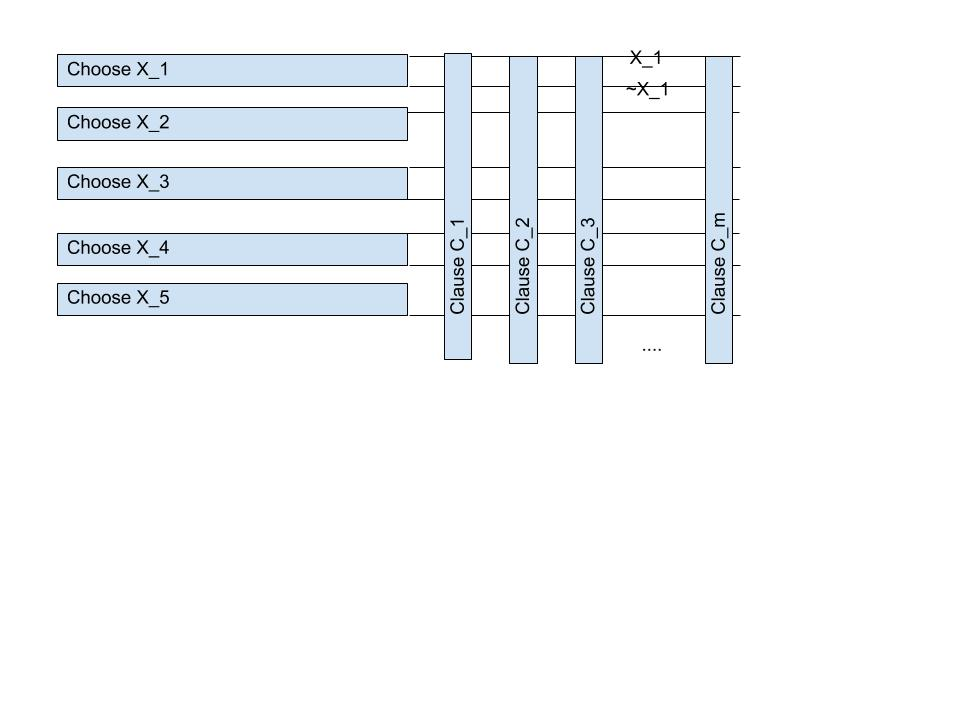
\includegraphics[width=\linewidth]{segment_apx_sketch.jpg}
\caption{\textbf{General schema.}}
General layout of VARIABLE-gadget and CLAUSE-gadget and how they
interact with each other.

TODO: Rename Choose X to VARIABLE-gadget and Clause C to CLAUSE-gadget.
\label{fig:segment_apx_sketch}
\end{figure}

We define:
$$\points := \bigcup_{1 \le i \le n} \pointsVar_i \cup \pointsClause_i $$
$$\sets := \bigcup_{1 \le i \le n} \segmentsVar_i \cup \segmentsClause_i $$

The subsequent sections define these sets.

We prove some properties of different gadgets.
Every segment for a gadget will only cover points 
in this gadget (won't interact with any diferent gadget),
so we can prove lemmas \textit{locally}.


TODO: $y$ axis is increasing values downward on figures
(not upwards like in normal).


\subsection{Construction lemmas and proof of Lemma \ref{apxconstruction}}
\newcommand{\setCoverInstance}{(\points, \sets)}
\newcommand{\true}{\texttt{true}}
\newcommand{\false}{\texttt{false}}

In order to prove Lemma \ref{apxconstruction} we introduce some
auxiliary lemmas proving properties of the construction
described in the previous section.

Consider an instance $S$ of MAX-(3,3)-SAT of size $n$
with optimum solution satisfying $k$ clauses.
Let us construct an instance $\setCoverInstance$ of geometric set cover
as described in Section~\ref{construction_description}
for instance $S$ of MAX-(3,3)-SAT.

\begin{lemma}
	\label{construction_correctness}
	Instance $\setCoverInstance$ of geometric set cover
	admits a solution of size $15n - k$.
\end{lemma}

\begin{proof}
Let the clauses in $S$ be $c_1$,~$c_2$~$\ldots$~$c_n$
and variables be $x_1$,~$x_2$~$\ldots$~$x_n$.
Let the assignment of the variables in
the optimum solution to $S$ be
$\phi : \{ x_1, x_2 \ldots x_n\} \rightarrow \{\true, \false\}$.


We cover every VARIABLE-gadget with solution described in
Lemma~\ref{choose_variables_solution},
in the $i$-th gadget choosing the set of segments corresponding to the
value of $\phi(x_i)$.

For every clause that is satisfied, say $c_i$, 
let us name the variable that is $\true$ in it $x_i$
and point corresponding to $x_i$ in $\pointsClause_i$ as $a$.
Points in $\pointsClause_i$ 
are covered with set $\segmentsClauseSolTrue{a}_i$ described in
Lemma~\ref{cover_clauses_solution_true}.
For every clause that is not satisfied, say $c_j$,
points in $\pointsClause_j$ are covered
with set $\segmentsClauseSolFalse_i$ described in
Lemma~\ref{cover_clauses_solution_false}.

Formally we define 
sets responsible for choosing variable and satisfing the variable,
$R_i$ and $C_i$ respectively, as following:

\begin{align}
	\begin{split}
	& R_i = \begin{cases}
		\chooseVar_i^{true} & \text{if}\ \phi(x_i) = \true \\
		\chooseVar_i^{false} & \text{if}\ \phi(x_i) = \false \\
		\end{cases} \\
	& C_i = \begin{cases}
		\segmentsClauseSolTrue{a}_i & \text{if}\ c_i \text{ satisfied} \\
		\segmentsClauseSolFalse_i & \text{if}\ c_i \text{ not satisfied}
		\end{cases} \\
	& \sol = \bigcup\limits_{i=1}^{n} \{R_i \cup C_i : 1 \le i \le n\}.
    \end{split}
\end{align}


This set covers all the points from $\points$, because
the sets $R_i$, $C_i$ individually cover their corresponding gadgets,
as proved in respective lemmas.

All of these sets are disjoint, so the size of the obtained solution is:

$$|\sol| = \sum_{i=1}^{n} R_i + \sum_{i=1}^n C_i = 3n + 11k + 12(n-k) = 15n - k.$$
\end{proof}
\begin{lemma}
	\label{construction_completness}
	Suppose we have a solution $\sol$ of the instance $\setCoverInstance$
	of geometric set cover that is of size $w$.
	Then there exists a solution of $S$
	that satisfies at least $15n - w$ clauses.
\end{lemma}


\begin{proof}\leavevmode
Let the clauses in $S$ be $c_1$,~$c_2$~$\ldots$~$c_n$
and variables be $x_1$,~$x_2$~$\ldots$~$x_n$.
Given a solution $\sol$
of the instance $\setCoverInstance$ of geometric set cover,
we construct a solution of $S$ by constructing an
assigment of variables 
$\phi : \{ x_1, x_2 \ldots x_n\} \rightarrow \{\true, \false\}$
that satisfies at least $15n-w$ clauses in $S$.

\subparagraph{Variables}
The solution $\sol$ needs to use at least 3 segments
to cover $\pointsVar_i$
for each VARIABLE-gadget (Lemma~\ref{choose_variables_no_less}).
If $\sol$ contains both segments $\xTrueSegment{i}$ and $\xFalseSegment{i}$,
then it has used at least 4 segments (Lemma~\ref{choose_variables_both}).


\begin{align}
	\begin{split}
	& \begin{cases}
	|\mathsf{pointsVar}_i \cap \sol| \ge 4 & \text{if}\ \xTrueSegment{i} \in \sol \land \xFalseSegment{i} \in \sol \\
	|\mathsf{pointsVar}_i \cap \sol| \ge 3 & \text{otherwise}
	\end{cases}
	\end{split}
\end{align}

We will now create modified solution $\sol'$ such that $|\sol'|=|\sol|$
and $\sol'$ is still a correct solution for $\setCoverInstance$.

If $\sol$ contains at most one of the segments $\xTrueSegment{i}$ and $\xFalseSegment{i}$,
choose the corresponding variable value to the constructed assignment $\phi$.
If $\sol$ contains none of these segments, set value to \false.
If $\sol$ contains both segments,
assign the value $\phi(x_i)$ that satisfies most clauses
in which $x_i$ occurs.
Every variable is in exactly 3 clauses,
so one assignment satisfies at least 2 of them.
In this case we remove one of the segments $\xTrueSegment{i}$
or $\xFalseSegment{i}$ (depending on the value of $\phi(x_i)$)
from $\sol'$ and replace it
with a segment that covers the point $v_{j,1}$
for a CLAUSE-gadget for a clause $c_j$ that uses $x_i$ with value $\neg\phi(x_i)$

Formally, we define the value $\phi(x_i)$ for the variable $x_i$ as follows:
\begin{align}
	\begin{split}
	\label{eqn:variable_assignment}
	& \begin{cases}
	\phi(x_i) = majority(X_i) & \text{if}\ \xTrueSegment{i} \in \sol \land \xFalseSegment{i} \in \sol \\
	\phi(x_i) = \true & \text{if}\ \xTrueSegment{i} \in \sol \\
	\phi(x_i) = \false & \text{if}\ \xFalseSegment{i} \in \sol \\
	\phi(x_i) = \false & \text{otherwise}
	\end{cases}
	\end{split}
\end{align}

and $\sol'$ as:

TODO: This is not a correct mathematical notation, but I am not sure
how to define it clearly

\begin{align}
\sol' = \sol 
	\begin{split}
	& \begin{cases}
	- \{ \xFalseSegment{i} \} \cup \{ \orTrueSegment{j}{1} \}
	& \phi(x_i) = \true \land \text{if}\ \xTrueSegment{i} \in \sol \land \xFalseSegment{i} \in \sol \land \\
	& \text{clause } c_j \text{ is satisfied by } \phi(x_i) = \false \\
	- \{ \xTrueSegment{i} \} \cup \{ \orTrueSegment{j}{1} \}
	& \phi(x_i) = \false \land \text{if}\ \xTrueSegment{i} \in \sol \land \xFalseSegment{i} \in \sol \land \\
	& \text{clause } c_j \text{ is satisfied by } \phi(x_i) = \true, \\
	\end{cases}
	\end{split}
\end{align}

therefore $|\mathsf{pointsVar}_i \cap \sol'| \ge 3$ for every $i$.

\subparagraph{Clauses}

For a clause $C_i = x \lor y \lor z$,
$\sol'$ needs to use at least 11 segments to cover $\pointsClause_i - \{x, y, z\}$
in CLAUSE-gadget (Lemma~\ref{cover_clauses_segments_no_less}).

TODO: maybe put something with cases and names of sets as above

Moreover, if all of the points $\{x_{i,0}, y_{i,0}, z_{i,0}\}$
are not covered by the segments from $\sol' \cap \pointsVar_i$,
then $\sol'$ needs to cover $\pointsClause_i$
with at least 12 segments
by Lemma~\ref{cover_clauses_segments_no_less}.


TODO: Maybe remove section below, because we do this calculation at the end anyway
We covered CLAUSE-gadget with at least 11 or at least 12 segments:
$$|\bigcup\limits_{i=1}^n \segmentsClause_i \cap \sol'| \ge 11n + b$$
where $b$ is the number of clauses
where none of the segments covering the points $x_{i,0}, y_{i,0}, z_{i,0}$ were chosen
in $P_{var}^j$.

\subparagraph{Satisfied clauses with chosen variable assignment.}

Consider a clause, say $c_i$. If none of
the points $x_{i,0}, y_{i,0}, z_{i,0}$ in $\pointsClause_i$ were covered by
segments from $\sol' \cap \segmentsVar_j$,
this clause is not satisfied by assignment $\phi$.

If one of these points is covered by 
segments from VARIBALE-gadget (TODO better this or $\sol' \cap \segmentsVar_j$),
then denote this point as $t$ and say it corresponds to variable $x_j$.
Consider the cases of choosing value of $\phi(x_j)$
in equation \eqref{eqn:variable_assignment}.

If $\sol'$ contains only one of the segments $\xTrueSegment{j}$ and $\xFalseSegment{j}$,
then the value $\phi(x_j)$ satisfies $c_i$.

If $\sol'$ contains neither $\xTrueSegment{j}$ nor $\xFalseSegment{j}$,
then it is impossible that $t$ is covered by segments in $\sol \cap \segmentsVar_j$.

$\sol'$ was chosen in such a way, that it is impossible that it contains
both $\xTrueSegment{i}$ and $\xFalseSegment{i}$ for some variable $i$.

This means that $\phi$ satisfies all but at most $a$ clauses in $S$.


To conclude, we proved that given a solution to $\setCoverInstance$ of size $w$,
we have constructed a variables assignment $\phi$
that satisfies at least $n-a$ clauses of $S$.
Finally, note that

$$w \ge 3n + 11(n-a) + 12a = 3n + 11n + a = 14n + a,$$
hence
$$15n - w  \le 15n - 14n - a = n - a.$$

So $\phi$ satisfies at least $15n-w$ clauses of $S$.
\end{proof}

We are ready to conclude the proof of Lemma $\ref{apxconstruction}$.

\begin{proof}[Proof of Lemma \ref{apxconstruction}]
By Lemma~\ref{construction_correctness}, we know
that there exists a solution to $\setCoverInstance$ of size $15n-k$, so: 
$$opt(\setCoverInstance) \le 15n - k.$$
Since the optimum solution of $S$ satisfies $k$ clauses,
then according to Lemma~\ref{construction_completness}:
$$opt(\setCoverInstance) \ge 15n -k.$$
Therefore, the solution given by Lemma~\ref{construction_correctness} 
of size $15n - k$ is an optimum solution to the instance $\setCoverInstance$.
\end{proof}
